%#!uplatex main.tex

\section{Preparation}

In this section, we introduce basic prerequisites to understand
Iterated Inversion System (IIS.)

In this paper, we mainly work on circle or sphere inversions.

\subsection{Kleinian Groups}

Kleinian groups is discrete sub-group of the M\"obius transformation
groups. Visualized images of Kleinian groups often have fractal structures.

\subsection{M\"obius Transformations and Inversions}

M\"obius transformations are defined in the extended complex plane,
$\hat{\mathbb{C}} = \mathbb{C} \cup \{\infty\}$ and expressed as linear
fractional transformation
$f(z)=\frac{az + b}{cz + d}$, where $a,~b,~c,~d,~z \in \hat{\mathbb{C}}$.
However, it is also known that we can construct them out of a finite
composition of inversions. For more details, see the introduction of \cite{mobius}.

M\"obius transformations are classified into three types as loxodromic,
parabolic, or elliptic.
Loxodromic transformations have two fixed points and are conjugate to
scaling by complex numbers except for scaling by unit complex numbers.
Those whose multiplier is a positive real number
are also called hyperbolic transformations.
Parabolic transformations have one fixed point and are conjugate to
parallel translations.
Elliptic transformations have two fixed points and are conjugate to rotations.

An inversion in a circle
is defined as $f(z) = \frac{r^2}{~\overline{z - c}~} + c$, where $c$ and
$r$ are center and radius of the circle.
Note that an inversion in a circle with infinite radius is the same as
a reflection over a line.
Also, sphere inversion can be derived from a similar equation, and an inversion
in a sphere with infinite radius is the same as
a reflection through a plane.

%% \subsection{Transformation Groups}
%% describe transformation groups, generator, snd word

\subsection{Basic Methods for Visualization}

\begin{figure}[htbp]
  \center
  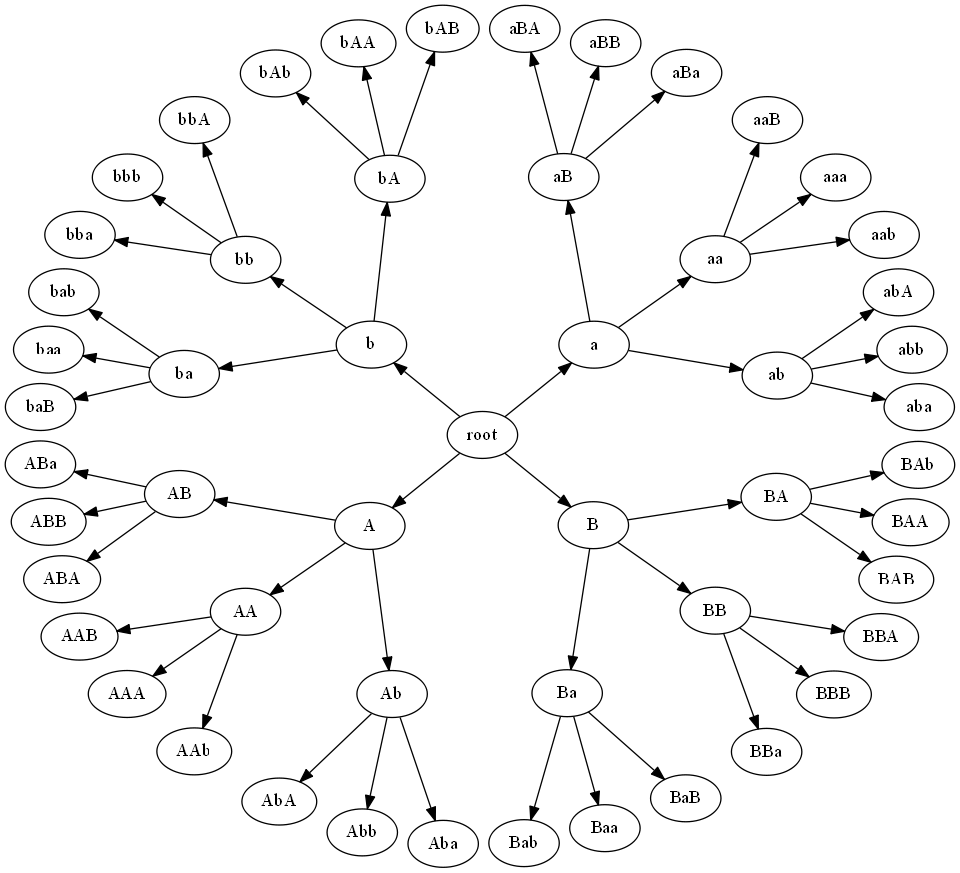
\includegraphics[height=1.35in, keepaspectratio]{img/cayleyGraph.png}
  \caption{\textit{Cayley Graph}}
  \label{fig:cayleyGraph}
 \hspace*{\fill}
\end{figure}

In this section, we introduce basic methods for visualizing Kleinian groups.
We consider \textit{cayley graph} of the Kleinian groups to enumerate elements
of the groups.
Figure \ref{fig:cayleyGraph} shows Cayley graph of Kleinian groups. The nodes of the graph
represent compositions of elements of the group.

There are two ways to visualize transformation groups.

Firstly, we can draw orbit of the group by traversing the cayley graph with
breadth first search.
We prepare fundamental tile, then apply found words.
See Figure n.
%% 種となる図に対し,探索で得られた語を作用させることで,その図の群によ
%% る軌道を描画することができる

Secondly, we can draw the limit set of the group by traversing the
cayley graph with depth first search.
We use fixed points of the groups.
we apply obtained word to the fixed points.
%% 極限集合はケーリーグラフの無限遠に存在している.そのため,固定点を用
%% いる.
%% 各固定点に探索で得られた語を作用させる

There are some faults in these methods.
For example, if we increase the number of generators,
It takes too much time to traverse the graph because of
combinatorial explosion.
Also, We have to traverse all of the graph
even though we don't need images outside of the screen.
This is the reason why we need other methods to visualize Kleinian
groups.
For more details about the methods, read Indra's Pearls.

%% ここからは行列表現ではなく円や球の反転を用いてクライン群を描画する.
%% 円や球には幾何学的な直観が働くため,行列そのものを扱うよりは非常にわ
%% かりやすい.

\subsection{Iterated Inversion System (IIS)}

\begin{figure}[htbp]
 \begin{minipage}[t]{0.16\hsize}
  \center
  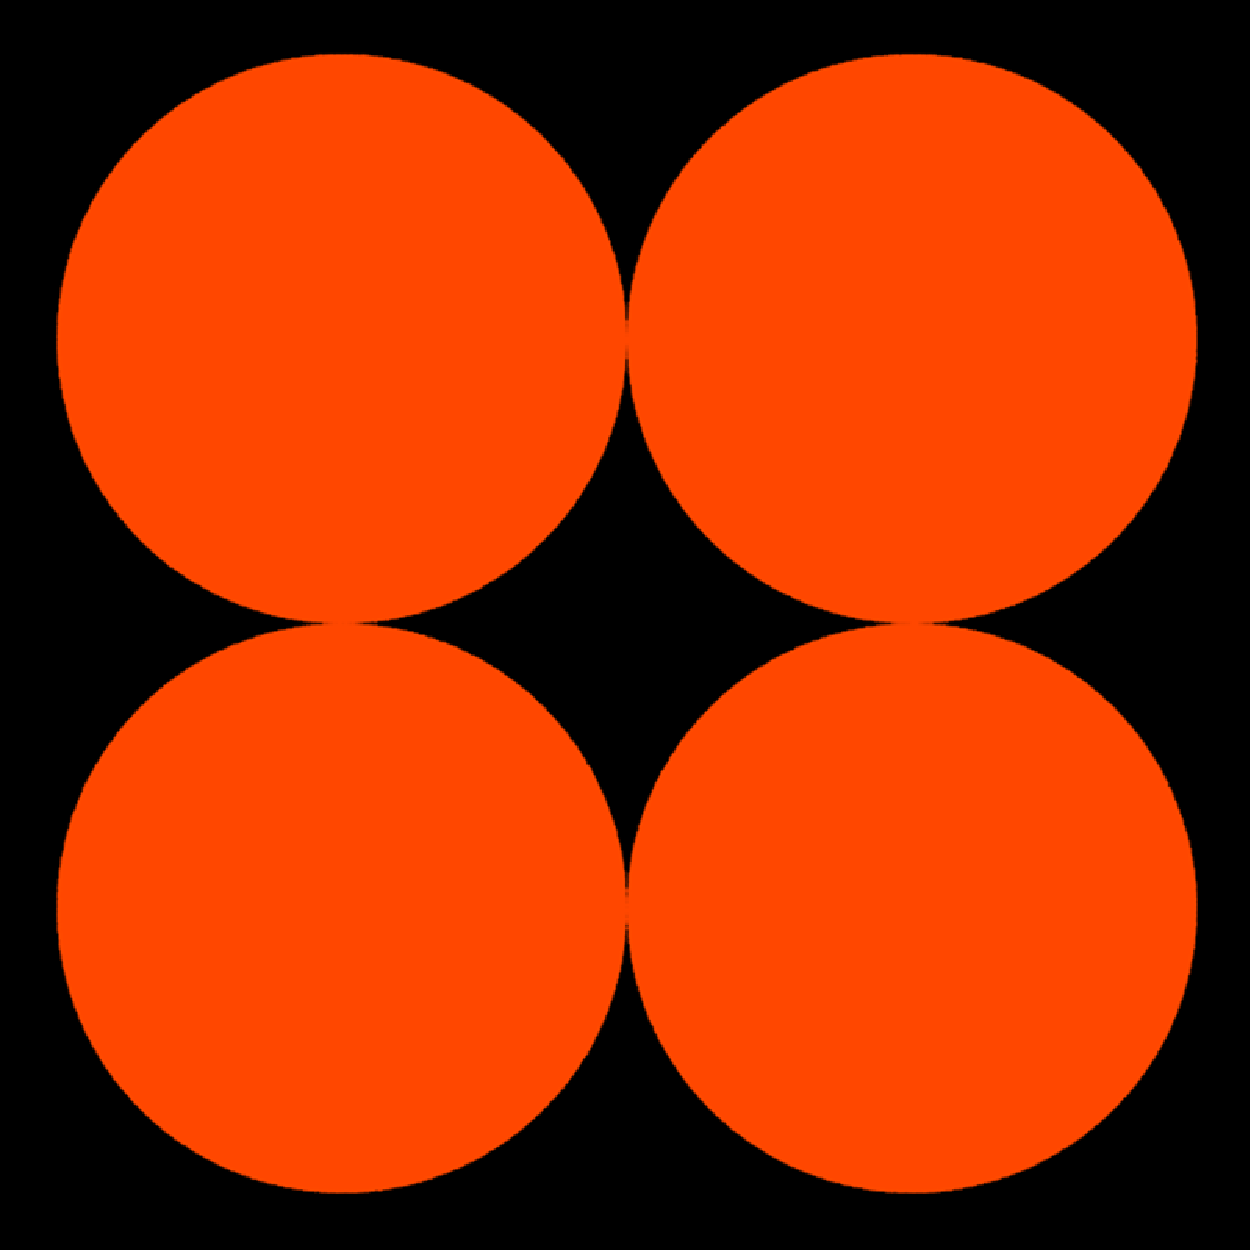
\includegraphics[width=1in, height=1in, keepaspectratio]{./img/preparation/orbit/level0c.pdf}
  \subcaption{}
  \label{fig:level0}
 \end{minipage}
 \begin{minipage}[t]{0.16\hsize}
  \center
  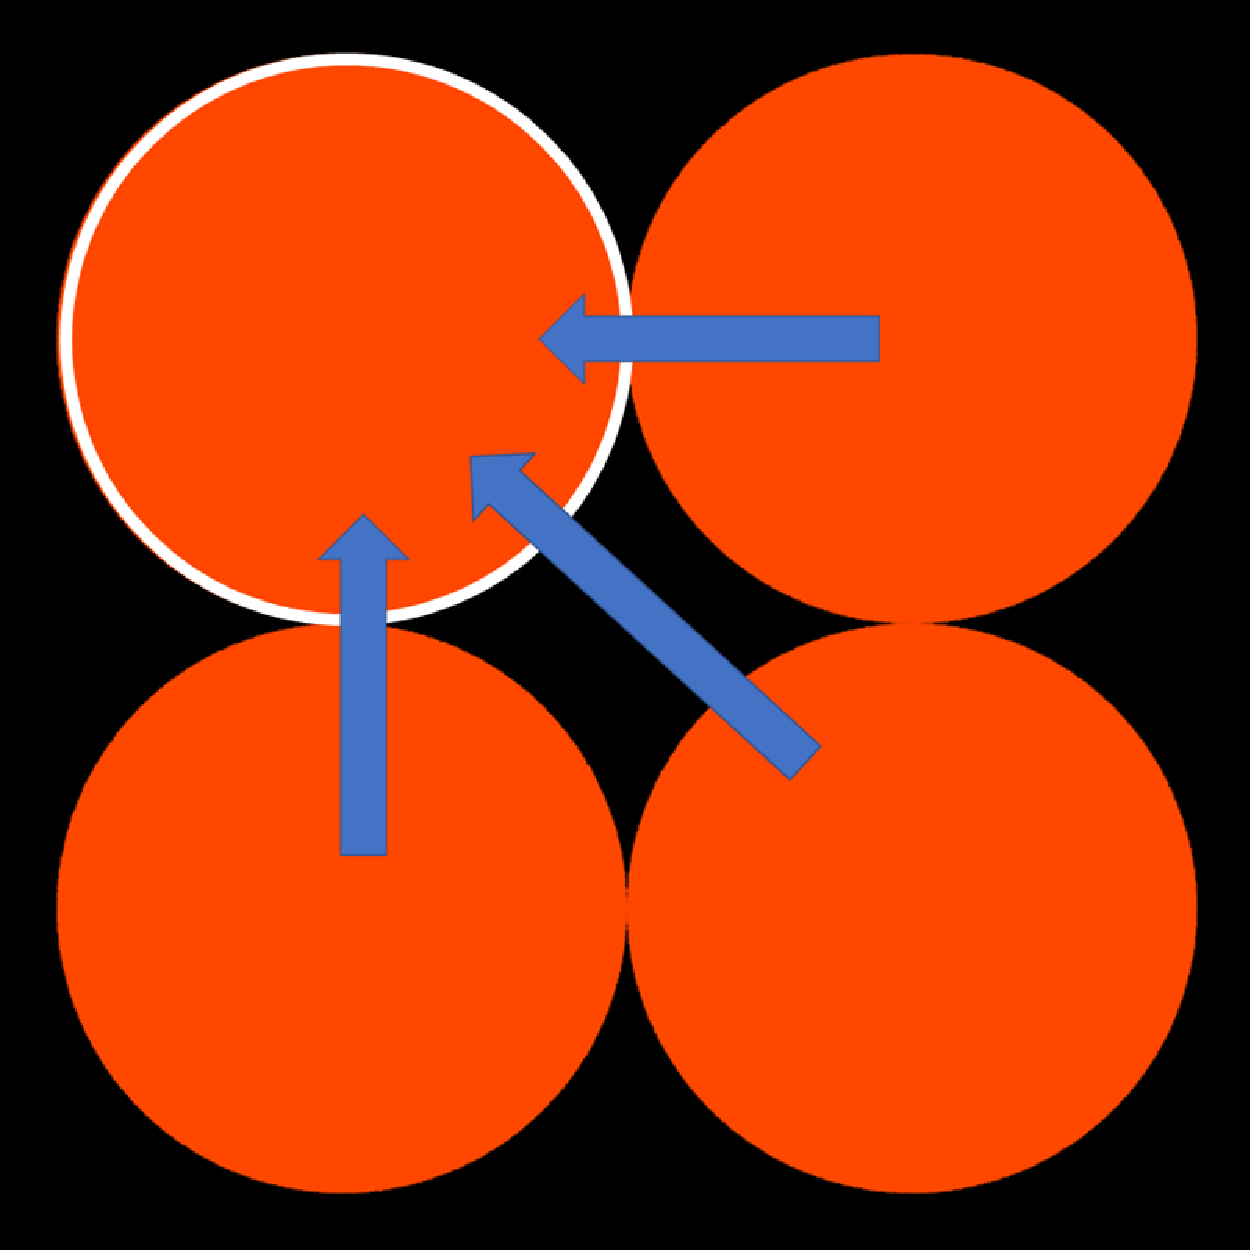
\includegraphics[width=1in, height=1in, keepaspectratio]{./img/preparation/orbit/level0invc.pdf}
  \subcaption{}
   \label{fig:level0inv}
 \end{minipage}
 \begin{minipage}[t]{0.16\hsize}
  \center
  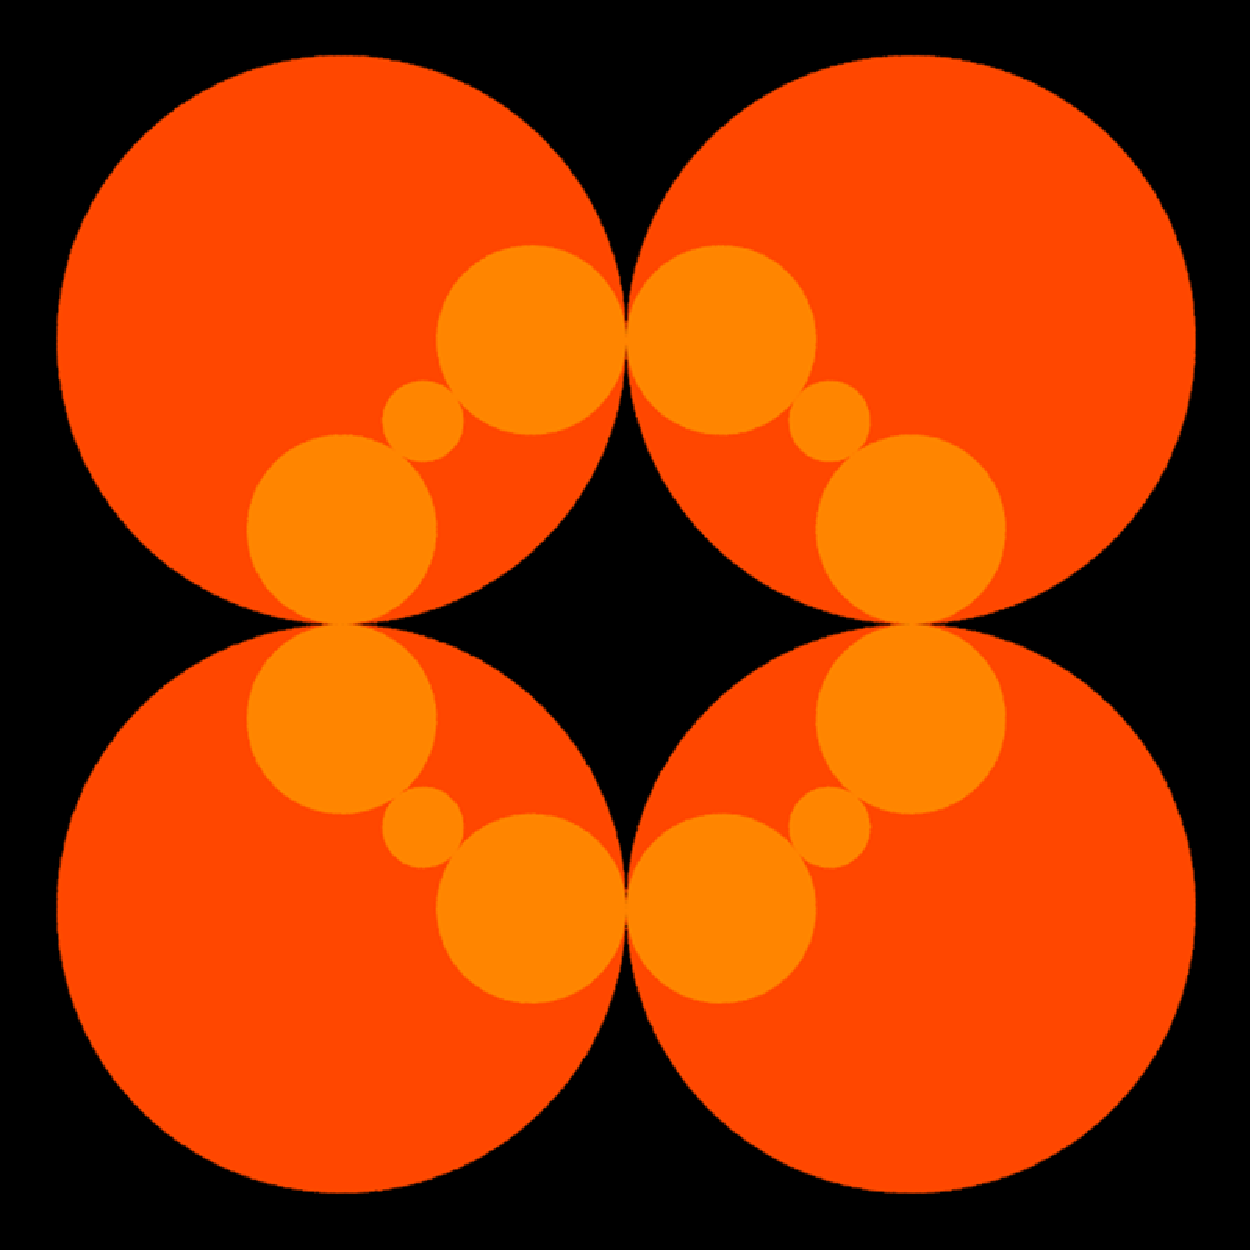
\includegraphics[width=1in, height=1in, keepaspectratio]{./img/preparation/orbit/level1c.pdf}
  \subcaption{}
   \label{fig:level1}
 \end{minipage}
 \begin{minipage}[t]{0.16\hsize}
  \center
  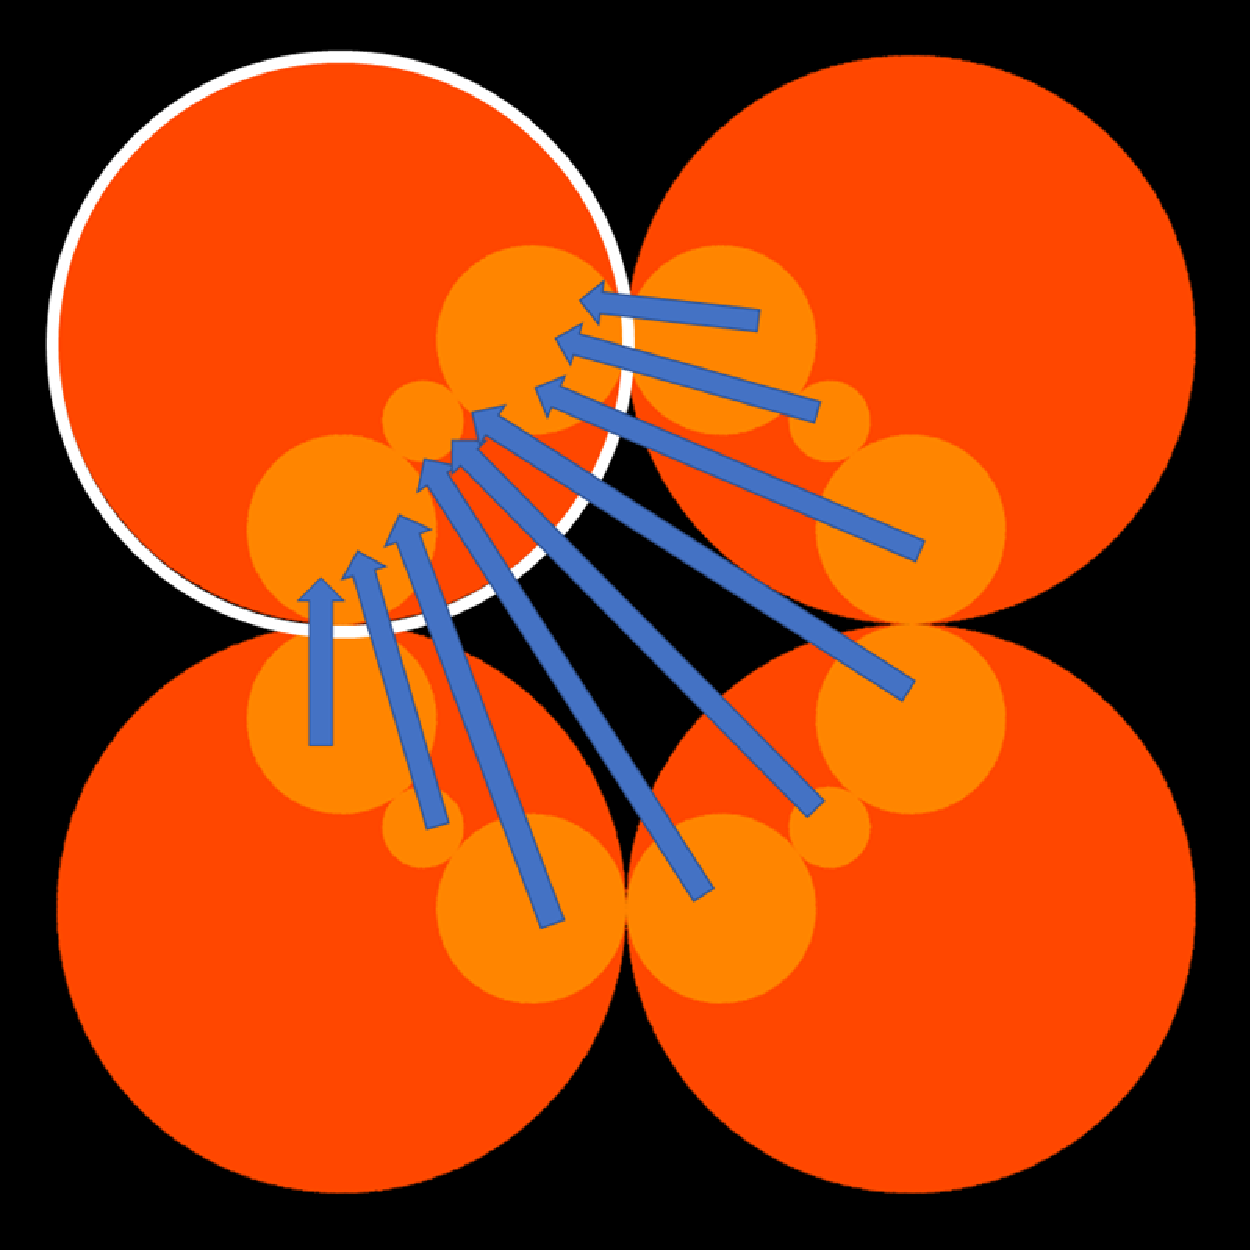
\includegraphics[width=1in, height=1in,
  keepaspectratio]{./img/preparation/orbit/level1invc.pdf}
  \subcaption{}
  \label{fig:level1inv}
 \end{minipage}
 \begin{minipage}[t]{0.16\hsize}
  \center
  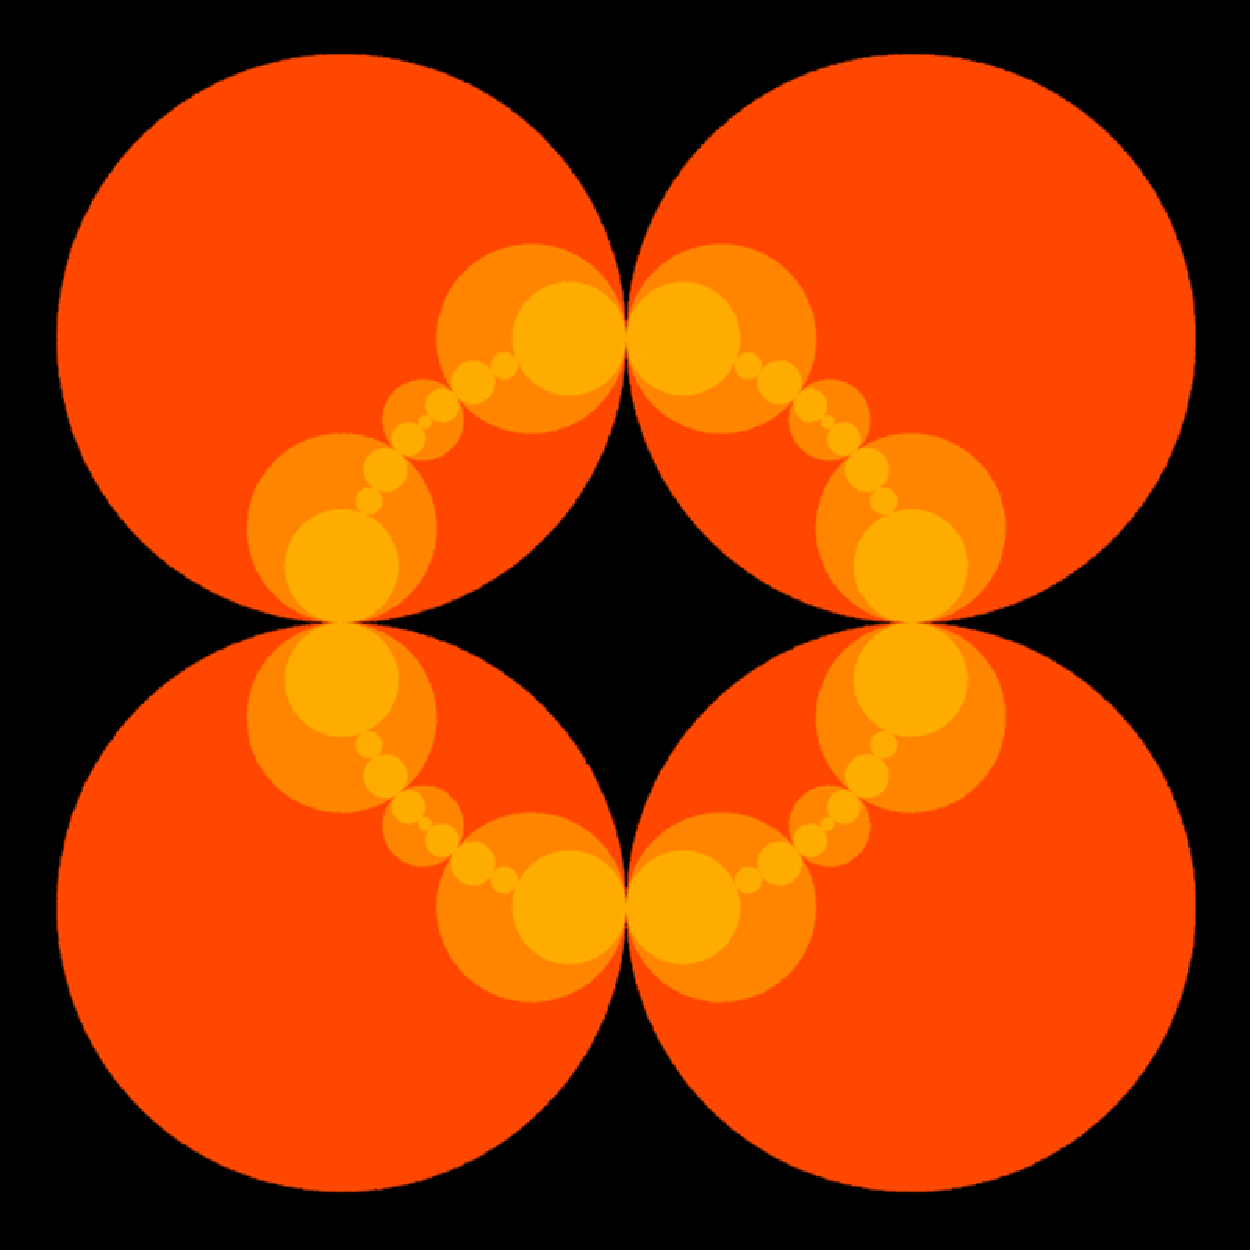
\includegraphics[width=1in, height=1in, keepaspectratio]{./img/preparation/orbit/level2c.pdf}
  \subcaption{}
  \label{fig:level2}
 \end{minipage}
 \begin{minipage}[t]{0.16\hsize}
  \center
  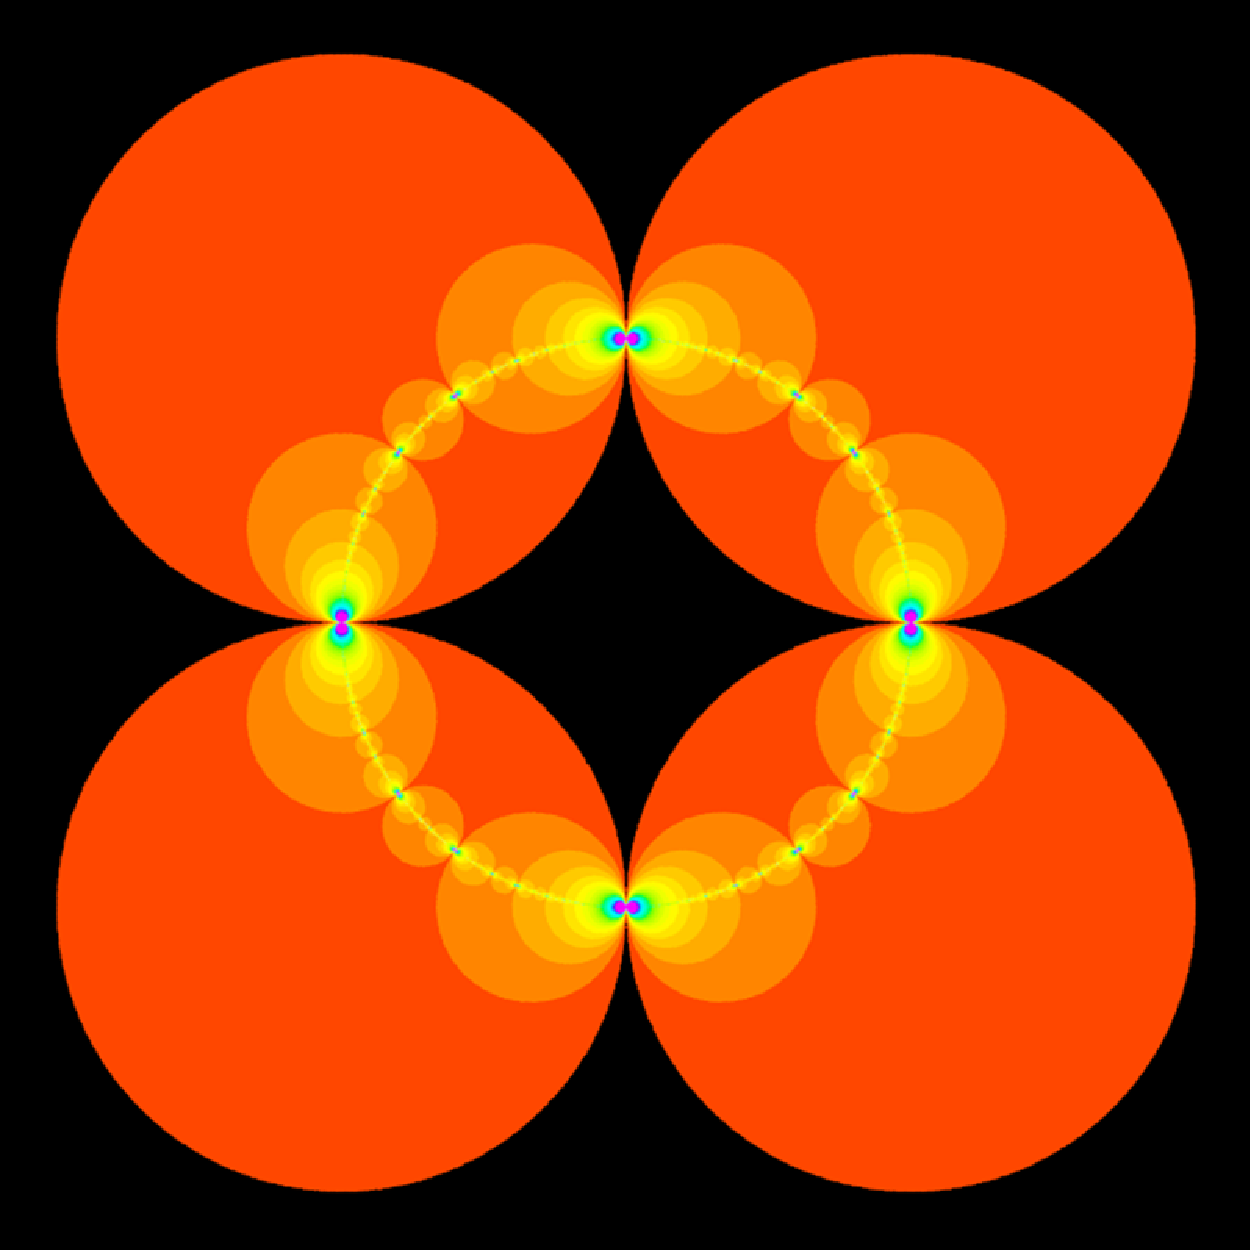
\includegraphics[width=1in, height=1in, keepaspectratio]{img/preparation/orbit/levelMaxc.pdf}
  \subcaption{}
  \label{fig:levelMax}
 \end{minipage}
 \caption{\textit{The process of rendering the orbit of Schottky disks}}
\end{figure}

To solve the problems we discussed in previous section,
we invent an efficient algorithm to visualize \textit{circle inversion
fractals} shown in Figure \ref{fig:levelMax}. 
The algorithm is called \textit{Iterated Inversion System (IIS.)}
The fractal is also Kleinian group composed of four circle inversions.
The fractal in Figure \ref{fig:levelMax} shows the orbit of the first
four circles.

The algorithm can visualize not only two dimensional ones but
also three dimensional sphere inversion fractals.

\subsubsection{Two Dimensional}

For two dimensional fractaks, the algorithm is as follows. 

The algorithm computes the depth of the circles pixel by pixel.
Thus, we can use parallel processing.
The images in this paper are rendered using \textit{OpenGL Shading
Language (GLSL)}.

%% Iterated Inversion Systemを考案した.特定のクライン群を高速に描画する
%% アルゴリズムである.これは二次元だけでなく,三次元にも作用させること
%% ができる.
%% ピクセルごとに計算を行うことで並列計算が可能になり,非常に高速に描画
%% を行うことができる.この論文にある図はOpenGL Shading Language (GLSL)
%% を用いて描画した.

IIS is applied to each point on the plane and computes nesting depth of
the disk which contains the point.
The process of the algorithm is as follows.
First of all, if the point is contained in initial disks, we invert the
point in the boundary circle of the disk.
We continue applying inversions until the transformed point is in the
out side of the initial circles.

inversions are involution. Thus we can 
%% 二次元のCircle Inversion Fractals を対象としてアルゴリズムを解説する.
%% 各点に関して関して,その点が反転円に属している際に,その円に関する反
%% 転を作用させる.これを移された点が全ての円の外側に出るまで繰り返す.
%% ここで,反転を作用した回数が,その点が含まれている円の深さである.ま
%% た,点の軌道上において各点の色を取得することで,絵の軌道を描画するこ
%% ともできる.
%% この手法は,円に関する反転が対合であることをうまく利用している.

\subsubsection{Three Dimensional Extension}

%% 二次元と同様に描画すると球が球の内側に連なってしまい,描画するのが難
%% しくなってしまう.例えばこれを描画するために, volume rendering という
%% 手法があるが,描画に時間がかかるうえ,得られる図もあまり面白くない.
%% そこで,二次元同様にもの(球)をおいてその軌道を描画するように変更した.

In the similar manner to two dimensional algorithm,
we extend the IIS to visualize three-dimensional kleinian groups.
We extend circle to sphere easily.

voxel by voxel.
and they are volume data.

The spheres are nesting

ray tracing 

volume rendering using \textit{ray marching}.
This is not efficient algorithm, and resulting images are not interesting.


We use \textit{Sphere Tracing} to render Three dimensional
fractals.
Sphere Tracing is one of the algorithm to ray tracing

\subsection{Related Works}

Aaron Montag
%% テクスチャベースの描画方法 テクスチャに種となる円を描き,円に変換を作
%% 用させることで極限集合を描画させる

Jos Leys
%% IISを普通の関数を使って行っている こちらのIISは円,球に注目している

Martin von Gagern introduce similar algorithm called \textit{Reverse
Pixel Lookup}. The algorithm is for visualizing tiling.